\documentclass[default]{beamer}
\setbeamertemplate{navigation symbols}{}

\usetheme{CambridgeUS}
\useoutertheme{infolines}
%\usecolortheme{crane}

\usepackage[utf8]{inputenc}					% Выбор языка и кодировки
\usepackage[english, russian]{babel}	% Языки: русский, английский
\usepackage{csquotes}
\usepackage{tikz}
\usetikzlibrary{arrows,shapes,calc}
\usepackage{animate}
\usepackage{fp}
\usepackage{textpos}

\usepackage[
	language=auto,
	autolang=other,
	backend=biber,
	style=authortitle,
	sorting=ydnt,
	maxbibnames=5
]{biblatex}
\addbibresource{strl_cai16.bib}
				
\DeclareSourcemap{
	\maps[datatype=bibtex, overwrite]{
		\map{
			\step[fieldset=langid, fieldvalue=english]
			\step[fieldset=doi, null]
			\step[fieldset=issn, null]
			\step[fieldset=isbn, null]
			\step[fieldset=url, null]
			\step[fieldsource=language, fieldset=langid, origfieldval]
		}
	}
}
\DeclareBibliographyDriver{std}{%
	\usebibmacro{bibindex}%
	\usebibmacro{begentry}%
	\usebibmacro{author/editor+others/translator+others}%
	\setunit{\labelnamepunct}\newblock
	\usebibmacro{title}%
	\newunit\newblock
	\usebibmacro{maintitle+booktitle}
	\newunit\newblock
	\usebibmacro{journal}%
	\newunit\newblock
	\usebibmacro{date}%
	\newunit\newblock
	\usebibmacro{finentry}
}
\DeclareBibliographyAlias{article}{std}
\DeclareBibliographyAlias{book}{std}
\DeclareBibliographyAlias{inproceedings}{std}
\DeclareBibliographyAlias{incollection}{std}

\graphicspath{{../../images/}} 			% Пути к изображениям

\makeatletter
\setbeamertemplate{footline}
{
	\leavevmode%
	\hbox{%
		\begin{beamercolorbox}[wd=.333333\paperwidth,ht=2.25ex,dp=1ex,center]{author
				in head/foot}%
			\usebeamerfont{author in
				head/foot}\insertshortauthor~~\beamer@ifempty{\insertshortinstitute}{}{(\insertshortinstitute)}
		\end{beamercolorbox}%
		\begin{beamercolorbox}[wd=.333333\paperwidth,ht=2.25ex,dp=1ex,center]{title in
				head/foot}%
			\usebeamerfont{title in head/foot}\insertshorttitle
		\end{beamercolorbox}%
		\begin{beamercolorbox}[wd=.333333\paperwidth,ht=2.25ex,dp=1ex,right]{date in
				head/foot}%
			\usebeamerfont{date in head/foot}\insertshortdate{}\hspace*{2em}
			\insertframenumber{}\hspace*{2ex} 
		\end{beamercolorbox}
	}%
	\vskip0pt%
}

\addtobeamertemplate{frametitle}{}{
	\begin{textblock*}{100mm}(\textwidth-55pt,-23pt)
		
\includegraphics[width=2cm]{misc/logos/frccsc.png}
	\end{textblock*}
}

\newcommand{\predmatr}[3]{
	\node[ell, rectangle, minimum height = 15, minimum width = 7.5]  at (#1 pt,#2 pt) {}; 
	\node[ellf, rectangle, minimum height = 15, minimum width = 7.5] at (#1+7.5 pt,#2 pt) {};
	\node[minimum height = 15, minimum width = 15] (#3) at (#1+3.3pt,#2 pt) {};
	\draw[ell] (#1+7.5 pt,#2+7.5 pt) -- (#1 +7.5 pt,#2-7.5 pt);
}
\renewcommand*{\bibfont}{\tiny}
\setlength\bibitemsep{-5pt}

\begin{document}
	
	\title[STRL архитектура]{STRL: многоуровневая архитектура управления интеллектуальным агентом}
	\author[Макаров, Панов, Яковлев]{Макаров Д.А., Панов А.И., Яковлев К.С.}
	\institute[ИСА РАН]{Институт системного анализа\\Федерального исследовательского центра <<Информатика и управление>>\\Российской академии наук}
	\date{6 октября -- КИИ 2016} 
	
	\begin{frame}
		\titlepage
		\centering
		\par\bigskip\tiny Исследование выполнено при поддержке Российского научного фонда
		(проект № 14-11-00692)
		
		
\includegraphics[width=100pt]{misc/logos/ras.png} \hspace{10pt}
		
\includegraphics[width=80pt]{misc/logos/frccsc.png} \hspace{10pt}
		
\includegraphics[width=60pt]{misc/logos/isa.png}
	\end{frame}
	
	\begin{frame}
		\frametitle{Картина мира субъекта деятельности}
		\scriptsize
		\onslide<1->{
			Картина мира субъекта деятельности - это представления субъекта о внешней среде, о своих собственных характеристиках, целях, мотивах, о других субъектах и операции (произвольные и непроизвольные), осуществляемые на основе этих представлений.
		}
		\onslide<2->{
			\par\smallskip
			Элементом картины мира является знак:
			\begin{itemize}
				\item в смысле культурно-исторического подхода Выготского-Лурии,
				\item выполняющий функции в соответствии с теорией деятельности Леонтьева.
			\end{itemize}
		}
		\onslide<3->{
			\begin{columns}
				\begin{column}{0.4\textwidth}
					\centering
					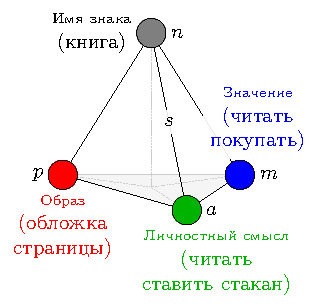
\includegraphics[width=0.6\textwidth]{signs/ru/sign_color_book_ru}
				\end{column}
		}
		\onslide<4->{
				\begin{column}{0.6\textwidth}
					\centering
					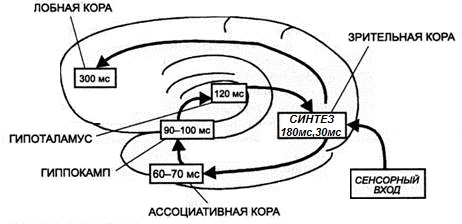
\includegraphics[width=0.6\textwidth]{misc/phisio/ivan_cyrc}
				\end{column}
			\end{columns}
			В пользу существования такой структуры свидетельствуют:
			\begin{itemize}
				\item нейрофизиологические данные (Эдельман, Иваницкий, Маунткастл и др.),
				\item другие психологические теории (например, трехкомпонентная модель Станович).
			\end{itemize}
			\vspace{-5pt}
			\nocite{*}
			\printbibliography[keyword={sign}, resetnumbers=true]
		}
	\end{frame}
	
	\begin{frame}
		\frametitle{Три образующих картины мира}
		\footnotesize
		\begin{figure}
			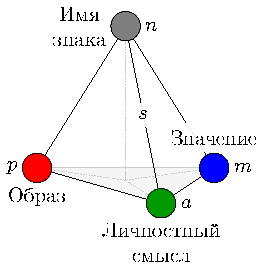
\includegraphics[width=0.3\textwidth]{signs/ru/sign_colored}
		\end{figure}
		
		Представляемая сущность описывается тремя причинно-следственными (каузальными) структурами:
		\begin{itemize}
			\item {\color{red}структура образа} - представление взаимосвязи внешних сигналов и внутренних характеристик субъекта (агента) - сенсо-моторное представление,
			\item {\color{blue}структура значения} - обобщенное знание о соотношениях во внешнем мире, согласованное в некоторой группе субъектов (агентов),
			\item {\color{green!60!black}структура личностного смысла} - ситуационная потребностно-мотивационная интерпретация знаний о соотношениях во внешней среде (значение для себя).
		\end{itemize}
	\end{frame}

	\begin{frame}
		\frametitle{Модель картины мира}
		
		\begin{columns}
			\begin{column}{0.55\textwidth}
				\begin{figure}
					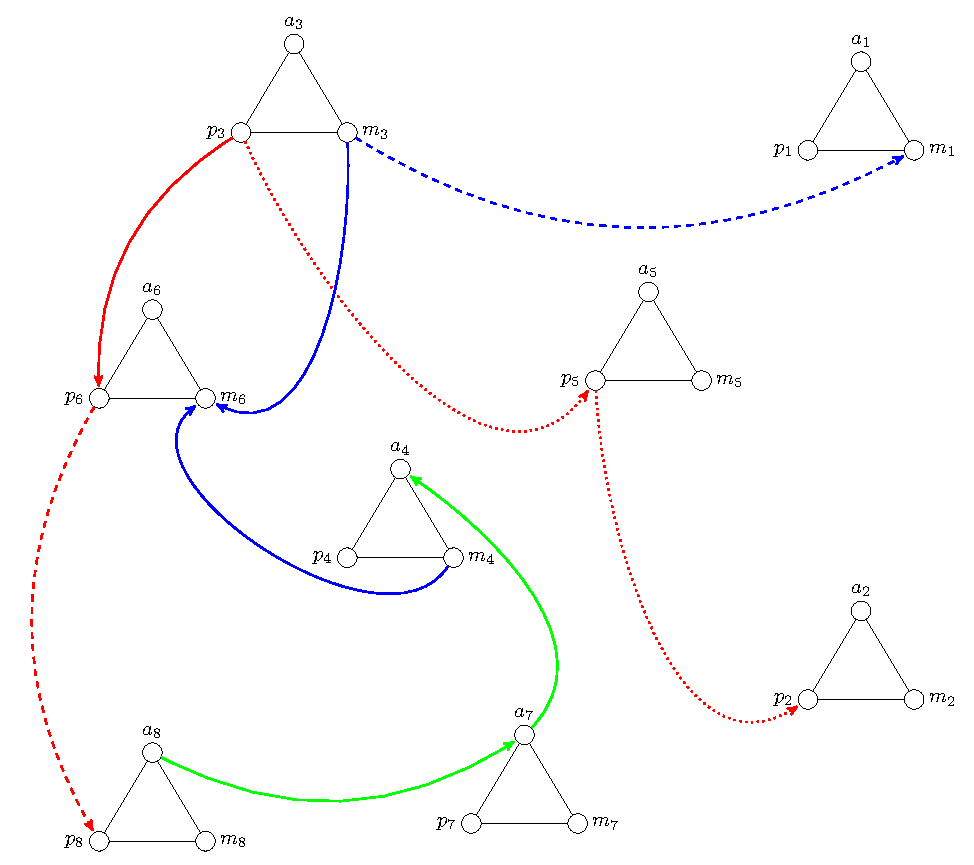
\includegraphics[width=\textwidth]{signnet/signs_net}
				\end{figure}
			\end{column}
			\begin{column}{0.45\textwidth}
				\textbf{Семиотическая сеть} - пятерка $\Omega=\langle W_p, W_m, W_a, R_n, \Theta \rangle$, где
				\begin{itemize}
					\item $W_p, W_m, W_a$ - соответственно каузальные сети на множестве образов, значений и личностных смыслах,
					\item $R_n$ - семейство отношений на множестве знаков, сгенерированных на основе трех каузальных сетей, т.е. $R_n=\{R_p, R_m, R_a\}$,
					\item $\Theta$ - семейство операций на множестве знаков.
				\end{itemize}
			\end{column}
		\end{columns}
		\nocite{*}
		\printbibliography[keyword={symbsign}, resetnumbers=true]
	\end{frame}	

	\begin{frame}
		\frametitle{Алгоритм планирования поведения}
		
		\begin{columns}
			\begin{column}{0.6\textwidth}
				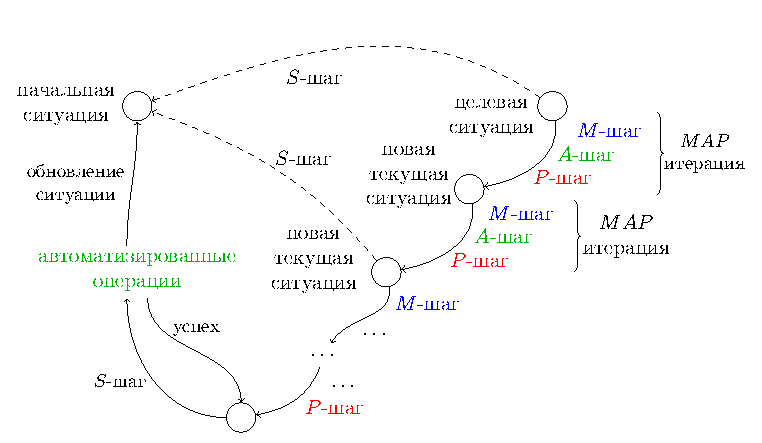
\includegraphics[width=\textwidth]{algo/ru/beh_plan2_ru}
				\vspace{20pt}
				\nocite{*}
				\printbibliography[keyword={plan}, resetnumbers=true]
			\end{column}
			\begin{column}{0.4\textwidth}
				\scriptsize
				Иерархический процесс планирования начинается с конченой ситуации и стремится достичь начальной ситуации.
				\par\bigskip
				MAP-итерация:
				\begin{itemize}
					\item \textit{M-step} -- поиск применимых действий на сети значений,
					\item \textit{A-step} -- генерация личностных смыслов, соответствующих найденным значениям,
					\item \textit{P-step} -- построение новой текущей ситуации по множеству признаков условий найденных действий,
					\item \textit{S-step} -- отправка сообщения другим участникам коалиции или выполнение найденного действия или активаций иерархии операция вплоть до автоматических операций.
				\end{itemize}
			\end{column}
		\end{columns}
		
	\end{frame}		

	\begin{frame}
		\frametitle{Задача интеллектуального перемещения}
		
		\begin{columns}
			\begin{column}{0.55\textwidth}
				\begin{center}
					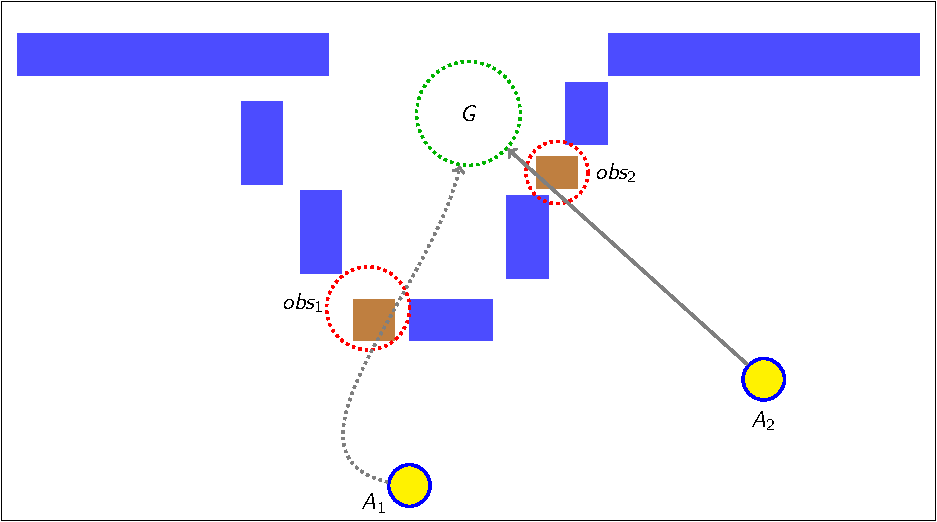
\includegraphics[page=1,width=0.8\textwidth]{examples/plan/slides_colored}
				\end{center}
				\vspace{-7pt}
				\small
				\textbf{Задача}
				
				Целевая область не достижима некоторым агентом самостоятельно (с использованием только методов планирования траектории).
				
				\textbf{Решение}
				
				Агенты должны поддерживать коммуникацию и модифицировать свои собственные планы с учетом коалиционных подзадач.
				
			\end{column}
			\begin{column}{0.45\textwidth}
				Особенности:
				\begin{itemize}
					\item Меняющаяся внешняя среда.
					\item Различные типы препятствий (некоторые могут быть разрушены).
					\item Агенты обладают различной функциональностью.
					\item Общая пространственная цель (ВСЕ агенты должны достичь определенной области на карте).
				\end{itemize}
			\end{column}
		\end{columns}
	\end{frame}

	\begin{frame}
		\frametitle{Архитектура агента}
		
		\centering
		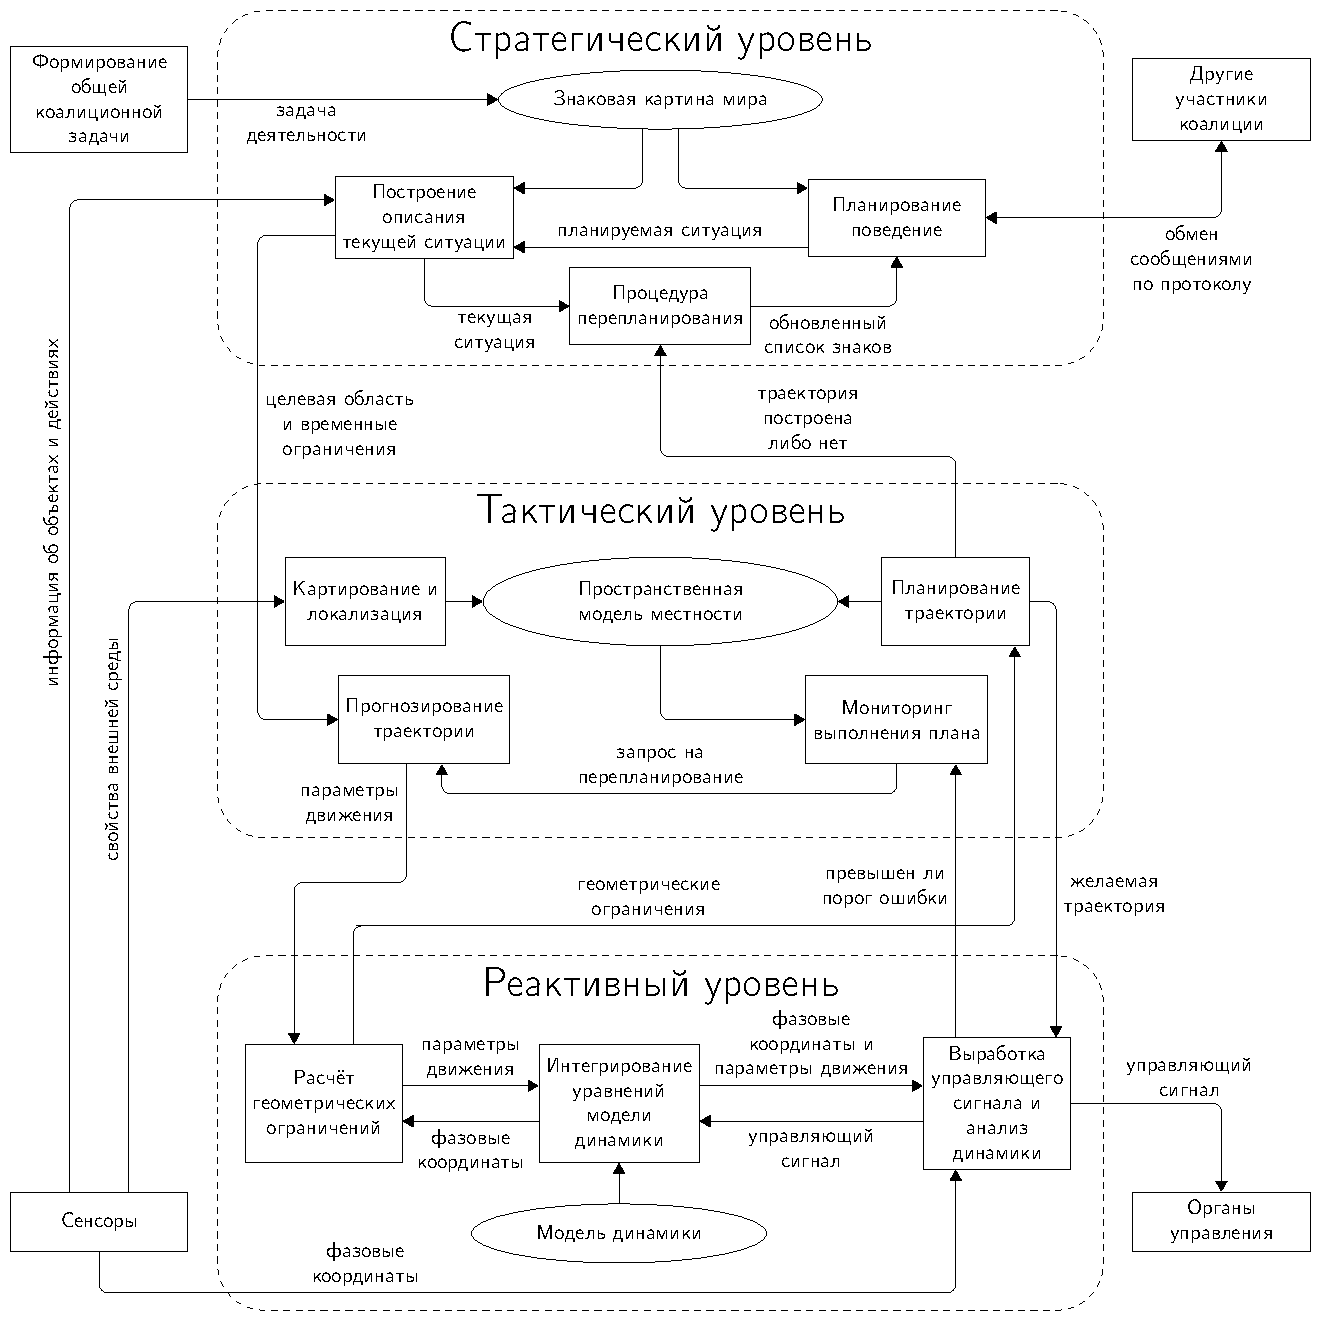
\includegraphics[width=0.5\textwidth]{agent-schemas/ru/architecture}

		\vspace{-5pt}
		\nocite{*}
		\printbibliography[keyword={strl}, resetnumbers=true]
	\end{frame}
		
	\begin{frame}
		\centering
		\Huge
		Спасибо за внимание!
		\normalsize
		\par\bigskip
		\par\bigskip
		ФИЦ ИУ РАН\\Лаборатория 0-2 <<Динамические интеллектуальные системы>>
		
		\par\bigskip
		pan@isa.ru, apanov@hse.ru
	\end{frame}			
\end{document}
	
	
